\documentclass[pdftex,12pt,a4paper]{article}
\pdfpagewidth 8.5in
\pdfpageheight 11.6in
\linespread{1.3}
\usepackage{anysize}
\marginsize{2.5cm}{2.5cm}{2.5cm}{2.5cm}

\usepackage[utf8]{inputenc}
\usepackage[T1]{fontenc}
%\usepackage[magyar]{babel}
\usepackage{indentfirst}
\usepackage{amsmath}
\usepackage{subcaption}
\usepackage{float}
\usepackage{graphicx}
\usepackage{braket}
\usepackage{tensor}
\usepackage{hyperref}

%\usepackage{listings}

\DeclareMathOperator{\Ai}{Ai}
\DeclareMathOperator{\Bi}{Bi}
\DeclareMathOperator{\Aip}{Ai^\prime}
\DeclareMathOperator{\Bip}{Bi^\prime}
\DeclareMathOperator{\Ti}{Ti}
\DeclareMathOperator{\ctg}{ctg}
\DeclareMathOperator{\sgn}{sgn}
%\DeclareMathOperator{\max}{max}
\let\Im\relax
\DeclareMathOperator{\Im}{Im}
\DeclareMathOperator{\Tr}{Tr}
\newcommand{\op}[1]{\hat{#1}}
\newcommand{\norm}[1]{\left\lVert #1 \right\rVert}
\newcommand*\Laplace{\mathop{}\!\mathbin\bigtriangleup}

\newcommand{\aeqref}[1]{\az{\eqref{#1}}}
\newcommand{\Aeqref}[1]{\Az{\eqref{#1}}}

%---------------------------------------------------------------------------------------------------------------------
\usepackage{fancyvrb,newverbs,xcolor}

\definecolor{cverbbg}{gray}{0.93}

\newenvironment{cverbatim}
 {\SaveVerbatim{cverb}}
 {\endSaveVerbatim
  \flushleft\fboxrule=0pt\fboxsep=.5em
  \colorbox{cverbbg}{\BUseVerbatim{cverb}}%
  \endflushleft
}
\newenvironment{lcverbatim}
 {\SaveVerbatim{cverb}}
 {\endSaveVerbatim
  \flushleft\fboxrule=0pt\fboxsep=.5em
  \colorbox{cverbbg}{%
    \makebox[\dimexpr\linewidth-2\fboxsep][l]{\BUseVerbatim{cverb}}%
  }
  \endflushleft
}

\newcommand{\ctexttt}[1]{\colorbox{cverbbg}{\texttt{#1}}}
\newverbcommand{\cverb}
  {\setbox\verbbox\hbox\bgroup}
  {\egroup\colorbox{cverbbg}{\box\verbbox}}
%---------------------------------------------------------------------------------------------------------------------
%\frenchspacing
\begin{document}

	\centerline{\bf\LARGE Comparing linear PDE solvers}\vskip0.4truein
	\centerline{\LARGE Computer simulations in physics}\vskip0.4truein
	\centerline{\Large\sc Kürti Zoltán}\vskip0.10truein
	%\centerline{\includegraphics[scale=0.5]{./elte_cimer_color.pdf}}
	\vskip0.4truein
	\centerline{\Large{\today}}
	\thispagestyle{empty}
	\newpage
	\tableofcontents
	\newpage
	\section{Introduction}
		Based on feedback about the last project, in this project I will be more focused on explaining my thought processes and motivations. I will also use more informal language as it is better suited to describe the journey I took while working with partial differential equations.
	\subsection{Motivation}
		The importance of numerically solving partial differential equations can hardly be overstated both in purely academic and engineering fields. At the same time I also like working on both partial and ordinary differential equations, this was one of the reasons my first project involved differential equations too. I dream about obtaining solutions for complicated situations in general relativity, but that's simply not feasible during a couple weeks, in fact I'm not even sure a single person could get meaningful results in this field. So I have to set realistic goals and the obvious first step is to start with a simple linear problem, like the heat equation.
		
		I also like to implement everything on my own, and I also like to come up with my own ideas even if I'm no the first to do so. This method takes a long time and generally isn't optimized for obtaining a result fast and with the less amount of energy. During evaluating a lab measurement to write the report or during a BSc. thesis the focus is on getting results in physics, not programming, and time is critical. In these situations usually people can't afford to begin the project by writing for loops, multiplications and additions in C, I certainly couldn't. This course however does focus on computer programming and writing low level algorithms. All in all this is the perfect opportunity for me to spend time on solving the heat equation on my own.
	\section{Solution outline}
		The first problem I thought about was calculating the laplacian on a discretized grid. This seemed to be an important and frequent operation while solving linear partial differential equations. While working on this problem I created the \ctexttt{coefficients.py} file. This file contains functions that help finding coefficients to approximate the laplacian at a point based on neighboring points up to different orders and with different conditions on the error terms. The functions generally work in $N$ dimensions, although the time for computations often grows exponentially with the number of dimensions. Some of the methods work for irregular grids, which would be very useful in case the discretization of a problem was matched to the geometry of the problem. I did not investigate this aspect, but it is a high priority extension I would make if I continue this project. With these functions it is possible to reproduce all the results about stencils in \cite{patra}, but my approach applies to irregular and also higher dimensional cases.
		
		The next step was to test some of these stencils I got from \ctexttt{coefficients.py}. I focused on one and two dimensional cases and compared single and double precision calculations too. Solving partial differential equations isn't just about choosing the right algorithms. A huge part of the process is finding optimal hyperparameters for the algorithm, like the resolution of discretization, the time step, relaxation parameters, precision of the floating point operations and so on. The choice of these parameters makes or breaks the success of the calculation. My impression so far is that there is no general rule for finding an optimal value for a parameter directly. Experimentation is needed, and this experimentation process can be sped up dramatically by good intuition. This part of the project certainly helped me to make more informed guesses during these types of experimentation.
		
		The last component to solve the first concrete problem is treating boundary conditions. My goal was to be able to handle arbitrary geometries both with Dirichlet and Neumann type boundary conditions. I did meat this goal in two dimensions and my solution generalizes to higher dimensions easily (adding one or two more nested for cycles depending on the function in question). The basic idea applies to irregular discretization, although in that case additional data structures would be needed to look up nearby points. To demonstrate this capability I solved the heat equation in a circle using a square grid for discretization with different combinations of Dirichlet and Neumann boundary conditions. \cite{gaussian,conduction}
	\section{Floating point precision}
		The speed of algorithms is critical for these problems. Especially as the dimension of the problem grows, discretization can quickly lead to millions of points, which need to be updated each time step. in a naiiv implementation calculating the laplacian on a grid is cache constrained. This is because each neighboring points only used a couple times (depending on the size of the stencil) before the calculation moves on and the element is replaced in the cache with other elements. Later in the next row this original value will have to be loaded again, if the rows are long enough. In my computer the L1 cache is $32kiB$. This is enough to hold $4096$ double precision floating point number. Using a 5x5 stencil for the laplacian to calculate each row the program has to load 5 rows of the original data, and the results of the calculation go to the L1 cache first too. Depending on the cache update policy even with a couple hundred elements long row elements may need to be loaded multiple times.
		
		This can be reduced by changing the order in which the laplacian is calculated. Instead of calculating it row by row, for large grids it may be more efficient to calculate the result in square chunks, designed to align with cache lanes ($64B$ on my computer) while maximizing the area of it with the constraint that it fits into the cache. This method would increase the number of uses a single value after each load and so would decrease the total amount of cache operations.
		
		Another great improvement could be the usage of single precision numbers. The discretization of the differential equation already introduces an error that can easily be bigger than single precision. Therefore to store the results of a calculation it ia probably enough to use single precision floating point numbers. The problem comes when the change of the solution is slow compared to the grid resolution (which is a desirable property if we want to minimize the error caused by discretization). The difference of two close floating point numbers will have a large error as the significant digits cancel out. This works against minimizing the discretization error. Increasing the precision of the number representation or using higher order approximations for the laplacian with smaller resolution may be two options to improve this situation.
	\subsection{Precision, step size and error order}
		\label{1dtest}
		In one dimension the laplacion of $f$ can be calculated as
		\begin{equation}
			\Laplace f_i = \frac{f_{i+1} - 2f_i + f_{i-1}}{h^2} + \mathcal{O}(h^4)
			\label{1laplace4}
		\end{equation}
		and as
		\begin{equation}
			\Laplace f_i = \frac{-\frac{1}{12}f_{i+2} + \frac{4}{3}f_{i+1} - \frac{5}{2}f_i + \frac{4}{3}f_{i-1} - \frac{1}{12}f_{i-2}}{h^2} + \mathcal{O}(h^6).
			\label{1laplace6}
		\end{equation}
		These expressions can be obtained from the taylor expansion of $f$ around $x_i$, this method will be discussed later more generally. In the first test program I calculated the laplacian of the sine function for different resolutions using equations \ref{1laplace4}. and \ref{1laplace6} both with single and double precision. The results are summarized in figure \ref{1dpdf}, the plot was made using the \texttt{1d.py} file and the data to be plotted was generated with the \texttt{1d64-32laplace} executable. The error on the figure is the biggest difference between the discretized laplacian and the analytic formula. The region on which the calculation was carried out is $2\pi$ long, and $N$ represents the number of points of the discretized grid.
		\begin{figure}[H]
			\centering
			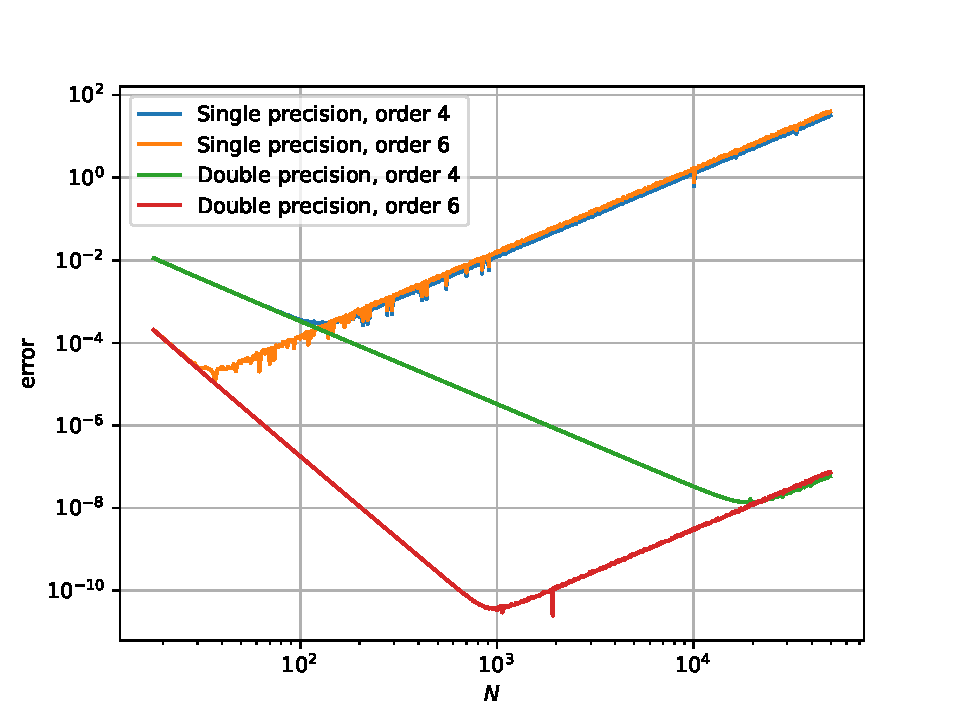
\includegraphics[scale=1]{./figs/1d.pdf}
			\caption{Error values of the discrete laplace for approximation with 4th and 6th order errors and single and double precision. }
			\label{1dpdf}
		\end{figure}
		It can be seen that there are two sources of error. One is the discretization error that decreases as $\frac{1}{N^4}$ or $\frac{1}{N^6}$. The other is the error coming from rounding error when two almost equal floating point numbers are subtracted. The key takeaway is that there is an optimum in precision, neither too big nor too small grid distances work. I observed similar behavior for two dimensional stencils as will be discussed later, and I expect the same for higher dimensions.
	\section{Higher order in many dimensions}
		Based on the above simple one dimensional case study, and as can be expected without any experiments, the most precise way to obtain the laplacian on a grid is using high precision floating point numbers and a finite difference approximation with higher order error terms. Obtaining the coefficients of these stencils becomes a non trivial task, and in the following section I will discuss my solution to this problem.
	\subsection{Designing the kernels}
		The code I will discuss can be found in the \texttt{coefficients.py} file. My strategy was the following. First, collect the displacements of the stencil points from the center. Since I only applied this method to stencils over a regular grid, this task was not difficult. Second, calculate the taylor polynomial corresponding to each point of the stencil. Third I searched for stencil coefficients with which multiplying the taylor expansion of grid points and summing the up gives the laplace operator up to a given order in derivatives. Finally, in case there are multiple such stencils, I further narrowed the stencil coefficients so that the leading order error term is a multiple of the power of the laplace operator. These stencils are called isotropic stencils. Their error due to discretization (in leading order) does not depend on the orientation of the grid. This provides additional stability in solving differential equations, especially in cases where the difference between neighboring grid points is considerable. I would like to describe some of the key elements of the algorithms laid out above.
		
		The first important structure is the taylor polynomial, used in many places in this code. It is represented by a list, each element of this list corresponds to a term in the taylor polynomial. Each term of the taylor polynomial is represented by a list, who's first element is the coefficient of the derivative, and the second term contains N integer numbers corresponding to the order of derivative in the $N$ different directions of the $N$ dimensional grid. The taylor polynomial corresponding to a stencil point is built up using $N$ repeated one dimensional taylor expansions. To do this I had to implement a polynomial multiplier function.
		
		Another important element of this file is the assumptions I made about the form of the stencils. First I assumed that they are symmetric to mirroring along each coordinate. This assumption works out because the laplace operator has this property. This assumption cancels out all the terms from the final result with odd derivatives. My second assumption was that it's symmetric under coordinate exchanges. This is a valid assumption, since exchanging coordinates is just a special case of a rotation or a rotation and a mirroring depending on the parity of the dimension.
		
		Solving for all the possible finite difference laplace operator is just a matter of solving linear set of equations, 
		\begin{equation}
			Ax_0=b,
			\label{Axb}
		\end{equation}
		where $A$ is the matrix that produces the coefficients of the taylor polinom from the coefficients of the stencil. With a particular solution and a matrix $C$ who's columns span the null space of $A$ all of the stencil coefficients that give the laplace operator up to the specified order are of the form
		\begin{equation}
			x = x_0 + Ct,
			\label{laplaceCoeffs}
		\end{equation}
		where $t$ is a parameter vector.
		
		The last calculation this file does is from this group of solutions choose the ones that are isotropic. These solutions are determined by the equation
		\begin{equation}
			A(x_0 + Ct) - b = \alpha b^{n}.
		\end{equation}
		$b^{n}$ are the taylor coefficients of the laplace operator to the $n$th power. This equation can be solved by multiplying the equation by a $P = I - b^{(n)} \circ b^{(n)} / b^{(n)} \cdot b^{(n)}$ projection matrix. This gives
		\begin{equation}
			PCt = - PAx_0 + Pb.
		\end{equation}
		The solution for $t$ from this equation is in general an affine space, similar to the situation in equation \ref{Axb}. These solutions determine the isotropic finite difference approximations of the laplace operator.
	\subsection{Testing the stencils}
		I picked three small stencils from the results of the previous section, and repeated a similar test to \ref{1dtest}. The difference was that this time I used a gaussian function as a test function, although I found that the results are not changed significantly as long as the test function has non zero higher order derivatives.The result is shown in figure \ref{2dpdf}.
		\begin{figure}[H]
			\centering
			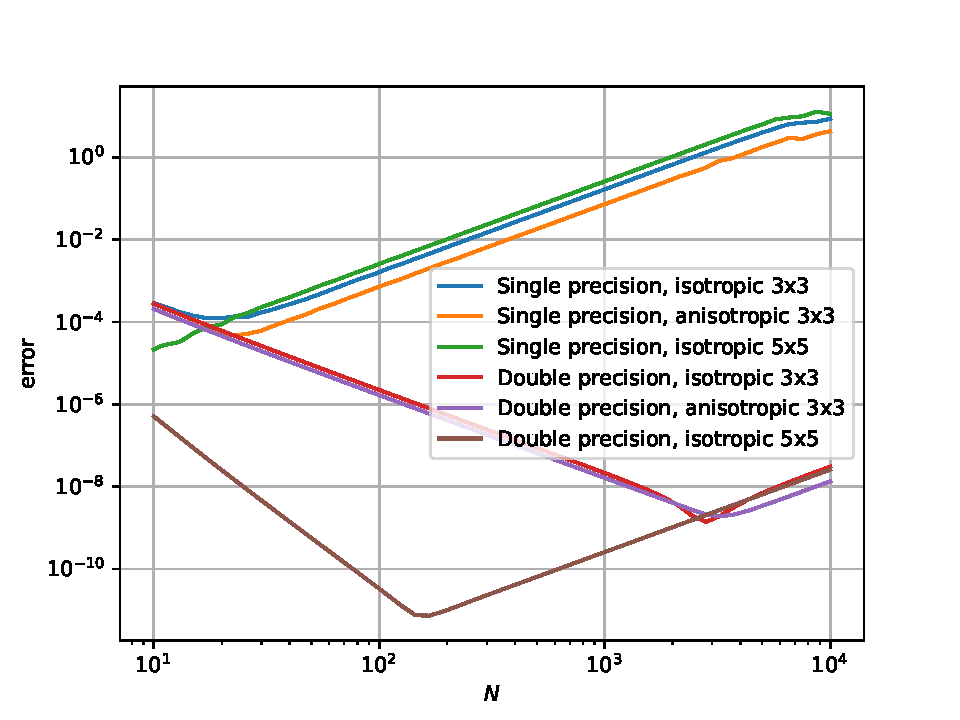
\includegraphics[scale=1]{./figs/2d.pdf}
			\caption{The error of different laplace stencils as a function of the discretization.}
			\label{2dpdf}
		\end{figure}
		The stencils I choose were
		\begin{equation}
			\begin{aligned}
			S_3^{iso} =& 
				\begin{bmatrix}
					\frac{1}{6} & \frac{2}{3} & \frac{1}{6}\\
					\frac{2}{3} & -\frac{5}{2} & \frac{2}{3}\\
					\frac{1}{6} & \frac{2}{3} & \frac{1}{6}\\
				\end{bmatrix},\\
			S_3^{ani} =&
				\begin{bmatrix}
					0 & 1 & 0\\
					1 & -4 & 0\\
					0 & 1 & 0\\
				\end{bmatrix},\\
			S_5^{iso} =& \frac{1}{60}
				\begin{bmatrix}
					0 & -2 & -1 & -2 & 0\\
					-2 & 16 & 52 & 16 & -2\\
					-1 & 52 & -252 & 52 & -1\\
					-2 & 16 & 52 & 16 & -2\\
					0 & -2 & -1 & -2 & 0\\
				\end{bmatrix}.\\
			\end{aligned}
		\end{equation}
		The plot was generated with the \texttt{2d.py} file, and the data for the plot was generated with the \texttt{2dlaplacetest} executable.
	\section{Boundary conditions, where numeric methods shine}
		With simple linear differential equations like the heat equation, the only case when they may not have a simple analytic solution if they have complex boundary conditions. There is no particular solution of a differential equation without boundary conditions so it is a central topic. In practice boundary conditions are often complicated, neither Dirichlet nor Neumann, so it is worth spending time working on it.
		
		As I was searching for how others treat boundary conditions, I got my inspiration from this website. \cite{lectureNotes} In the problem they used they had a straight boundary with Neumann condition. Thy satisfied it by mirroring the solution to the boundary, and using the mirrored elements while calculating the finite differences at the boundary. This method can't be easily generalized to curved or straight but not aligned boundaries. However while reading this page I realized that maybe I can simply change the values at the boundary, and only update the inner points of the region according to the finite difference version of the differential equation.
		
		To sum it up, my general strategy is that I update the inner points of the region based on the differential equation, and I calculate the values at the boundary so that the boundary conditions are satisfied with the updated inner points. For Dirichlet type boundary conditions this means just setting the value at the boundary to the boundary condition, for Neumann type boundary condition this means setting the boundary point to the average of the nearby inner points. This method can be easily generalized to implement more complicated boundary conditions.
		
		To make this happen I needed a way to tell outer, inner and boundary points apart. The outer points can be determined by a user with a function: if the function returns a positive value for the coordinates of the point, it is an outer point. Otherwise a point is at the boundary if one of it's eight neighboring points is an outer point. The rest of the points don't have outer points as neighbors, can be updated using a 3x3 laplace stencil, they are the inner points. In case a bigger stencil is used, some of the inner points still need to be updated with a smaller stencil. The code that implements this ideas is the \texttt{allocateBoundary} function in the \texttt{timeEvolution.cpp} file. It fills up an array made of 8 bit values. Outer points are marked with 0, boundary points with 1 and inner points with 2 or higher values, depending on how big the stencils are that can be used with them as a center point.
		
		Two concrete examples are simulated with this code. Both of them have a circle as their boundary. The first one has Neumann boundary condition everywhere, physically this means perfect insulation. The starting temperature function is an off centered gaussian distribution. The integral of the initial temperature distribution is determined by what we choose the final temperature to be for an infinitely precise solution. (If the integral of the initial temperature distribution outside the circle is small, that is. I integrated the gaussian distribution over the whole plane.) The temperature of the center of the circle oer time is plotted in figure \ref{timepdf}. In this simulation I choose the final temperature to be $10$, which is well approximated by the simulation. The video of the simulation is uploaded to YouTube. \cite{gaussian}
		\begin{figure}[H]
			\centering
			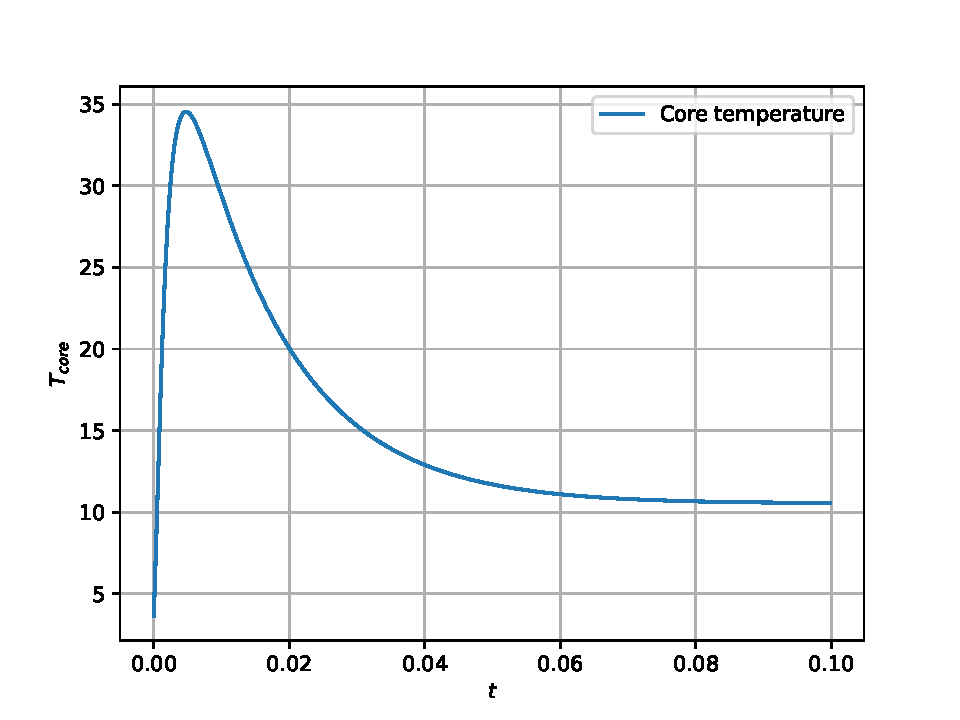
\includegraphics[scale=1]{./figs/time.pdf}
			\caption{The time dependence of the middle point.}
			\label{timepdf}
		\end{figure}
		
		The other example was in a circle too, with mostly Neumann boundary conditions. However, two symmetric sections are changed to Dirichlet boundary conditions, one with temperature 20, the other with temperature 0. The starting temperature distribution was constant 0. The animation of this simulation can also be viewed on YouTube. \cite{conduction}
	\section{Closing words}
		
	\bibliographystyle{abeld}
    \bibliography{ref}
\end{document}








